\documentclass[a4paper, 11pt]{article}

\usepackage[top=2cm, bottom=2cm, left=2cm, right=2cm]{geometry}
\usepackage[utf8]{inputenc}
\usepackage[T1]{fontenc}
\usepackage{indentfirst}

% Multiple columns
\usepackage{multicol}
\setlength{\columnseprule}{1pt} % separation line between columns

% Colors
\usepackage[usenames,dvipsnames]{xcolor}
\definecolor{dkgreen}{rgb}{0,0.6,0}
\definecolor{steelblue}{rgb}{0.16,0.37,0.58}
\definecolor{gray}{rgb}{0.5,0.5,0.5}
\definecolor{mauve}{rgb}{0.58,0,0.82}
\definecolor{blue}{rgb}{0,0,0.7}
\definecolor{hlColor}{rgb}{0.94,0.94,0.94}
\definecolor{shadecolor}{rgb}{0.96,0.96,0.96}
\definecolor{TFFrameColor}{rgb}{0.96,0.96,0.96}
\definecolor{TFTitleColor}{rgb}{0.00,0.00,0.00}
\definecolor{lightred}{rgb}{1,0.96,0.96}
\definecolor{darkred}{rgb}{0.85,0.33,0.31}
\definecolor{lightblue}{HTML}{EBF5FA}
\definecolor{lightblue2}{HTML}{E3F2FA}
\definecolor{darkblue}{HTML}{D2DCE1}
\definecolor{lightyellow}{HTML}{FFFAE6}
\definecolor{darkyellow}{HTML}{FAE6BE}

\usepackage{hyperref}
\hypersetup{
	colorlinks=true,	% false: boxed links; true: colored links
	linkcolor=black,	% color of internal links
	urlcolor=blue,		% color of external links
	citecolor=blue
}

% highlight
\usepackage{soul}
\sethlcolor{hlColor}

% Figures & graphics
\usepackage{graphicx}	% import graphics
\usepackage{wrapfig}	% wrap text around figures
\usepackage{subcaption} % subfigures

% Colored frames
\usepackage{mdframed}
\usepackage{framed}

\newenvironment{framehint}{%
	\begin{mdframed}[backgroundcolor=lightblue, linecolor=darkblue]%
}{\end{mdframed}}

\newenvironment{framehint2}{%
	\begin{mdframed}[backgroundcolor=lightblue2, linecolor=darkblue]%
}{\end{mdframed}}

\newenvironment{framewarning}{%
	\begin{mdframed}[backgroundcolor=lightyellow, linecolor=darkyellow]%
}{\end{mdframed}}

\newenvironment{frameurgent}{%
	\begin{mdframed}[backgroundcolor=lightred, linecolor=darkred]%
}{\end{mdframed}}

% Leftbar
\newlength{\leftbarwidth}
\setlength{\leftbarwidth}{1pt}
\newlength{\leftbarsep}
\setlength{\leftbarsep}{10pt}

\newcommand*{\leftbarcolorcmd}{\color{gray}}

\renewenvironment{leftbar}{%
    \def\FrameCommand{{\leftbarcolorcmd{\vrule width \leftbarwidth\relax\hspace {\leftbarsep}}}}%
    \MakeFramed {\advance \hsize -\width \FrameRestore }%
}{%
    \endMakeFramed
}

% Code listings
\usepackage{listings}
\lstset{
	language=C,
	basicstyle=\scriptsize,
	numbers=left,                   % where to put the line-numbers
  	numberstyle=\tiny\color{gray},
	commentstyle=\color{steelblue},
	stringstyle=\color{BrickRed},
	backgroundcolor=\color{shadecolor},
    keywordstyle=\color{OliveGreen},
	frame=single,                   % adds a frame around the code
 	rulecolor=\color{black},
	emph={},
	emphstyle=\color{mauve},
	morekeywords=[2]{},
	keywordstyle=[2]{\color{dkgreen}},
	showstringspaces=false,
  	tabsize=4,
	moredelim=[is][\small\ttfamily]{/!}{!/},
	breaklines=true
}

% Title page
\title{
	\textbf{INFOH414 - Swarm Robotics Project}\\
}
\date{\today}

\begin{document}
\maketitle
\newpage

\tableofcontents
\newpage

\section{Introduction}

The project consists of being able to move a swarm of robots from a central room
to the best neighbouring room. The four target rooms on each side of the central
room are evaluated based on the average of 3 metrics:

\begin{itemize}
    \item the \textbf{ground color} ($v_G \in [0,1]$),
    \item the \textbf{light intensity} ($v_L \in [0,1]$),
    \item the proportion of \textbf{objects} ($v_O \in [0,1]$ from the number
    of objects
$\in [2,12]$).
\end{itemize}

\noindent There are 2 types of robots, ground robots and light robots. Both of
them can evaluate the number of objects with an omnidirectional camera. Only the
ground robots can evaluate the ground color, and only the light robots can
evaluate the light intensity.\\

\noindent In order to attain the best room, the swarm must spread, evaluate rooms and
collectively decide on which is the best room.

\subsection{Project hierarchy}

\begin{framed}
\dirtree{%
.1 Project/.
.2 experiments/ - Output results.
.2 report/.
.2 scripts/ - Scripts to parse output results.
.2 src/.
.2 decision-making.xml - Argos configuration file.
.2 run.sh - Script to run 10 experiments sequentially.
.2 variables - Set the ARGOS\_PLUGIN\_PATH environment variable.
}
\end{framed}

\subsection {Build instructions}

\begin{lstlisting}
> mkdir build
> cd build
> cmake -DCMAKE_BUILD_TYPE=Release ../src/decision_making
> make
> cd ..
> source variables
> argos3 -c decision-making.xml
\end{lstlisting}

\newpage

\section{Idea \& Implementation}

\subsection{Idea}

\noindent The main idea can be split into the following steps (which also are
the states of the main controller, \hl{SwarmRobotics.lua}).

\begin{enumerate}
    \item Initialization
    \item Robots split into rooms by going to the nearest room. It does not
    ensure that a robot of each type will be in each room (see Analysis \&
    Problems section).
    \item Go towards target: light source for light robots, and door step for
    ground robots. Compute the 3 values to evaluate the room.
    \item Robots go towards farther robots in order to exit the current room.
    They group themselves inside the central room and share partial scores to
    obtain total score for their assignated room. Once total scores are computed,
    they can be shared to decide which is the best one.
    \item Go towards the best detected room.
\end{enumerate}

\subsection{Implementation details}

\subsubsection{MoveIntoRoom}

The \hl{MoveIntoRoom.lua} state machine has for purpose to let robots go towards
a room and detect when the robot is inside said room. First, the robot is
attracted by the door associated with the room. When the robot is close enough
to the door (1st threshold), then it is attracted by elements inside the room
(objects and light source). Once a 2nd threshold has been reached, the robot is
considered inside the room.

\subsubsection{TargetRoomFormation}

The \hl{TargetRoomFormation.lua} has for purpose to let robots go towards their
target once inside a room. Light robots go towards the light source and Ground
robots go towards the door step. Moreover, a vector reprensenting robots
interaction is computed using the Lennard-Jones force. This is done in order
to avoid robots blocking each other (repulsion), while keeping them close to
avoid unecessary wandering.

\subsubsection{EvaluateRoom}

\hl{EvaluateRoom.lua} lets robot evaluate their room. Light robots will evaluate
the light intensity and the number of objects, while ground robots will evaluate
the ground color. The evaluation is considered done when the partial score has
not been improved for a specific number of steps.\\

For the evaluation of objects, objects outside the current target room can be
detected. In order to avoid this situation, objects outside a 3m meter radius
around the robot are discarded.

\subsubsection{Message channels}

The following bytes have been reserved for the range\_and\_bearing system to
exchange messages (see \hl{MsgBytes.lua}).

\begin{enumerate}
    \item ping, notify position of current robot to other robots, used for
    pattern formation
    \item red, red component of a room's color
    \item green, green component of a room's color
    \item blue, blue component of a room's color
    \item L robot partial score (light intensity + objects evaluation)
    \item G robot partial score (ground evaluation)
    \item associated room's total score
\end{enumerate}

\subsection{Main steps}

\begin{figure}[h!]
        \centering
        \begin{subfigure}[b]{0.5\textwidth}
            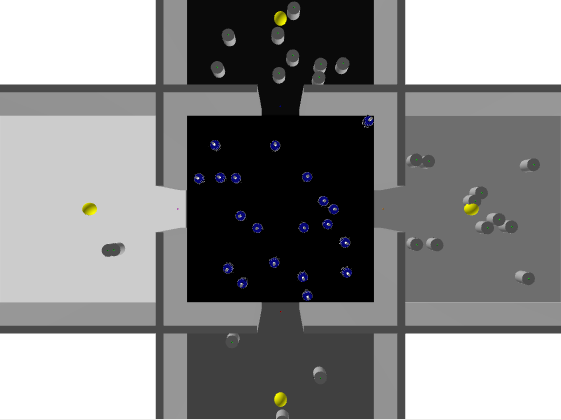
\includegraphics[width=\textwidth]{images/1_start.png}
            \caption{Start}
        \end{subfigure}%
        ~
        \begin{subfigure}[b]{0.5\textwidth}
            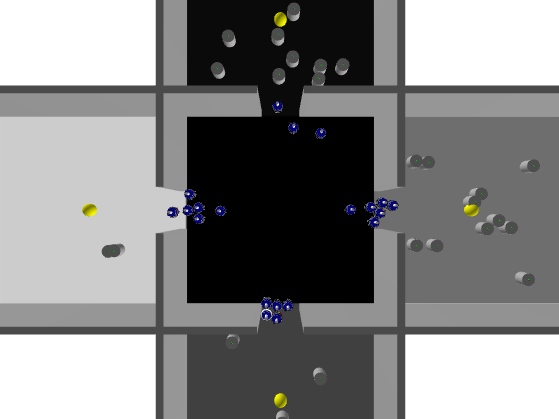
\includegraphics[width=\textwidth]{images/2_split.png}
            \caption{Split}
        \end{subfigure}
        \hfill
        \begin{subfigure}[b]{0.5\textwidth}
            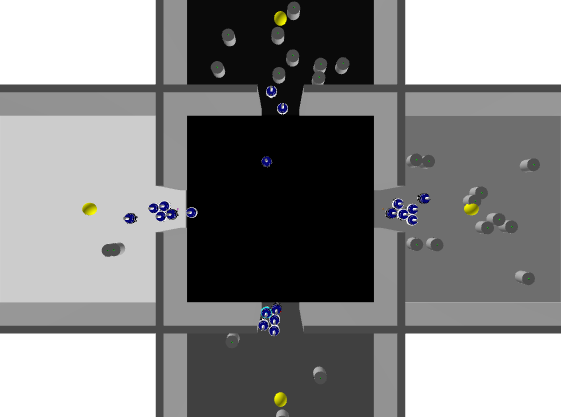
\includegraphics[width=\textwidth]{images/3_evaluate.png}
            \caption{Room evaluation}
        \end{subfigure}%
        ~
        \begin{subfigure}[b]{0.5\textwidth}
            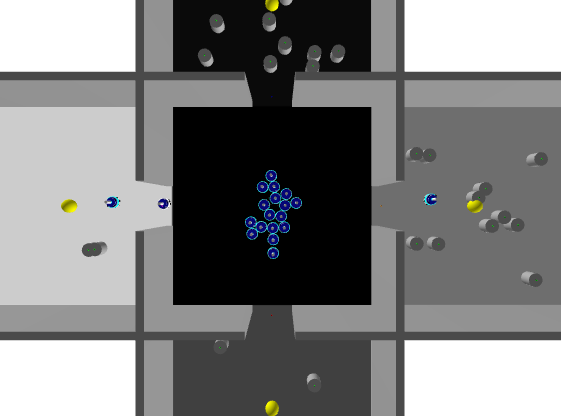
\includegraphics[width=\textwidth]{images/4_sync.png}
            \caption{Gathering \& scores sync}
        \end{subfigure}
        \hfill
        \begin{subfigure}[b]{0.5\textwidth}
            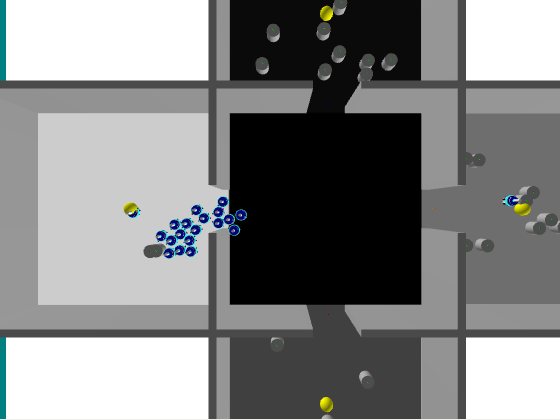
\includegraphics[width=\textwidth]{images/5_best.png}
            \caption{Go to best room}
        \end{subfigure}
        \caption{Main steps}\label{fig:steps}
\end{figure}

% TODO screenshots steps
\newpage

\section{Implementation}
% TODO

\newpage

\section{Analysis \& Problems}

\begin{table}[h]
\begin{tabular}{lllll}
\hline
\multicolumn{1}{|l|}{N}                   & \multicolumn{1}{l|}{$\rho$} & \multicolumn{1}{l|}{\begin{tabular}[c]{@{}l@{}}Average time\\ steps\end{tabular}} & \multicolumn{1}{l|}{\begin{tabular}[c]{@{}l@{}}Best room\\ chosen\\ (/number of\\ experiments)\end{tabular}} & \multicolumn{1}{l|}{\begin{tabular}[c]{@{}l@{}}Average \% of robots\\ in the chosen room\end{tabular}} \\ \hline
\multicolumn{1}{|l|}{20}                  & \multicolumn{1}{l|}{0.3}    & \multicolumn{1}{l|}{909}                                                          & \multicolumn{1}{l|}{6/10}                                                       & \multicolumn{1}{l|}{82.5\%}                                                                            \\ \hline
\multicolumn{1}{|l|}{}                    & \multicolumn{1}{l|}{0.5}    & \multicolumn{1}{l|}{779}                                                          & \multicolumn{1}{l|}{7/10}                                                       & \multicolumn{1}{l|}{96\%}                                                                              \\ \hline
\multicolumn{1}{|l|}{}                    & \multicolumn{1}{l|}{0.7}    & \multicolumn{1}{l|}{794}                                                          & \multicolumn{1}{l|}{5/10}                                                       & \multicolumn{1}{l|}{92\%}                                                                              \\ \hline
\multicolumn{1}{|l|}{\multirow{3}{*}{25}} & \multicolumn{1}{l|}{0.3}    & \multicolumn{1}{l|}{922}                                                          & \multicolumn{1}{l|}{5/10}                                                       & \multicolumn{1}{l|}{92.8\%}                                                                            \\ \cline{2-5}
\multicolumn{1}{|l|}{}                    & \multicolumn{1}{l|}{0.5}    & \multicolumn{1}{l|}{837}                                                          & \multicolumn{1}{l|}{7/10}                                                       & \multicolumn{1}{l|}{92\%}                                                                              \\ \cline{2-5}
\multicolumn{1}{|l|}{}                    & \multicolumn{1}{l|}{0.7}    & \multicolumn{1}{l|}{987}                                                          & \multicolumn{1}{l|}{5/10}                                                       & \multicolumn{1}{l|}{86\%}                                                                              \\ \hline
\multicolumn{1}{|l|}{\multirow{3}{*}{30}} & \multicolumn{1}{l|}{0.3}    & \multicolumn{1}{l|}{990}                                                          & \multicolumn{1}{l|}{8/10}                                                       & \multicolumn{1}{l|}{92.3\%}                                                                            \\ \cline{2-5}
\multicolumn{1}{|l|}{}                    & \multicolumn{1}{l|}{0.5}    & \multicolumn{1}{l|}{973}                                                          & \multicolumn{1}{l|}{6/10}                                                       & \multicolumn{1}{l|}{91.3\%}                                                                            \\ \cline{2-5}
\multicolumn{1}{|l|}{}                    & \multicolumn{1}{l|}{0.7}    & \multicolumn{1}{l|}{883}                                                          & \multicolumn{1}{l|}{6/10}                                                       & \multicolumn{1}{l|}{93.7\%}                                                                            \\ \hline
\multicolumn{1}{|l|}{35}                  & \multicolumn{1}{l|}{0.5}    & \multicolumn{1}{l|}{1166}                                                         & \multicolumn{1}{l|}{5/10}                                                       & \multicolumn{1}{l|}{87\%}                                                                              \\ \hline
\multicolumn{1}{|l|}{40}                  & \multicolumn{1}{l|}{0.5}    & \multicolumn{1}{l|}{1033}                                                         & \multicolumn{1}{l|}{7/10}                                                       & \multicolumn{1}{l|}{80.5\%}                                                                            \\ \hline
                                          &                             &                                                                                   &                                                                                 &                                                                                                        \\ \hline
\multicolumn{2}{|l|}{Total}                                             & \multicolumn{1}{l|}{934}                                                          & \multicolumn{1}{l|}{67/110}                                                     & \multicolumn{1}{l|}{89.6\%}                                                                            \\ \hline
\end{tabular}
\end{table}


% TODO analysis

% TODO problems
%   * no diversification
%       * ideas not implemented (or did not work well):
%           * assign robots randomly to rooms, evaluate, restart from beginning
%           of state machine multiple times
%           * room assignment at the beginning or the program
%   * multiple forces
%       * behaviour difficult to predict
%       * robots wandering outside rooms
%       * collisions (split vs gathering)
%   * more robots -> get stuck more easily

\newpage


\end{document}
